% Options for packages loaded elsewhere
\PassOptionsToPackage{unicode}{hyperref}
\PassOptionsToPackage{hyphens}{url}
%
\documentclass[
]{article}
\usepackage{lmodern}
\usepackage{amssymb,amsmath}
\usepackage{ifxetex,ifluatex}
\ifnum 0\ifxetex 1\fi\ifluatex 1\fi=0 % if pdftex
  \usepackage[T1]{fontenc}
  \usepackage[utf8]{inputenc}
  \usepackage{textcomp} % provide euro and other symbols
\else % if luatex or xetex
  \usepackage{unicode-math}
  \defaultfontfeatures{Scale=MatchLowercase}
  \defaultfontfeatures[\rmfamily]{Ligatures=TeX,Scale=1}
\fi
% Use upquote if available, for straight quotes in verbatim environments
\IfFileExists{upquote.sty}{\usepackage{upquote}}{}
\IfFileExists{microtype.sty}{% use microtype if available
  \usepackage[]{microtype}
  \UseMicrotypeSet[protrusion]{basicmath} % disable protrusion for tt fonts
}{}
\makeatletter
\@ifundefined{KOMAClassName}{% if non-KOMA class
  \IfFileExists{parskip.sty}{%
    \usepackage{parskip}
  }{% else
    \setlength{\parindent}{0pt}
    \setlength{\parskip}{6pt plus 2pt minus 1pt}}
}{% if KOMA class
  \KOMAoptions{parskip=half}}
\makeatother
\usepackage{xcolor}
\IfFileExists{xurl.sty}{\usepackage{xurl}}{} % add URL line breaks if available
\IfFileExists{bookmark.sty}{\usepackage{bookmark}}{\usepackage{hyperref}}
\hypersetup{
  pdftitle={Blossom Watch 2021},
  pdfauthor={Alan Millington},
  hidelinks,
  pdfcreator={LaTeX via pandoc}}
\urlstyle{same} % disable monospaced font for URLs
\usepackage[margin=1in]{geometry}
\usepackage{longtable,booktabs}
% Correct order of tables after \paragraph or \subparagraph
\usepackage{etoolbox}
\makeatletter
\patchcmd\longtable{\par}{\if@noskipsec\mbox{}\fi\par}{}{}
\makeatother
% Allow footnotes in longtable head/foot
\IfFileExists{footnotehyper.sty}{\usepackage{footnotehyper}}{\usepackage{footnote}}
\makesavenoteenv{longtable}
\usepackage{graphicx,grffile}
\makeatletter
\def\maxwidth{\ifdim\Gin@nat@width>\linewidth\linewidth\else\Gin@nat@width\fi}
\def\maxheight{\ifdim\Gin@nat@height>\textheight\textheight\else\Gin@nat@height\fi}
\makeatother
% Scale images if necessary, so that they will not overflow the page
% margins by default, and it is still possible to overwrite the defaults
% using explicit options in \includegraphics[width, height, ...]{}
\setkeys{Gin}{width=\maxwidth,height=\maxheight,keepaspectratio}
% Set default figure placement to htbp
\makeatletter
\def\fps@figure{htbp}
\makeatother
\setlength{\emergencystretch}{3em} % prevent overfull lines
\providecommand{\tightlist}{%
  \setlength{\itemsep}{0pt}\setlength{\parskip}{0pt}}
\setcounter{secnumdepth}{-\maxdimen} % remove section numbering

\title{Blossom Watch 2021}
\author{Alan Millington}
\date{2021-03-22 17:03:15}

\begin{document}
\maketitle

\begin{longtable}[]{@{}lr@{}}
\toprule
\begin{minipage}[b]{0.41\columnwidth}\raggedright
hashtag\strut
\end{minipage} & \begin{minipage}[b]{0.10\columnwidth}\raggedleft
count\strut
\end{minipage}\tabularnewline
\midrule
\endhead
\begin{minipage}[t]{0.41\columnwidth}\raggedright
blossom\strut
\end{minipage} & \begin{minipage}[t]{0.10\columnwidth}\raggedleft
2361\strut
\end{minipage}\tabularnewline
\begin{minipage}[t]{0.41\columnwidth}\raggedright
blossomwatch\strut
\end{minipage} & \begin{minipage}[t]{0.10\columnwidth}\raggedleft
1521\strut
\end{minipage}\tabularnewline
\begin{minipage}[t]{0.41\columnwidth}\raggedright
NationalTrust + BlossomWatch\strut
\end{minipage} & \begin{minipage}[t]{0.10\columnwidth}\raggedleft
36\strut
\end{minipage}\tabularnewline
\begin{minipage}[t]{0.41\columnwidth}\raggedright
EveryoneNeedsNature\strut
\end{minipage} & \begin{minipage}[t]{0.10\columnwidth}\raggedleft
267\strut
\end{minipage}\tabularnewline
\begin{minipage}[t]{0.41\columnwidth}\raggedright
None\strut
\end{minipage} & \begin{minipage}[t]{0.10\columnwidth}\raggedleft
1827\strut
\end{minipage}\tabularnewline
\bottomrule
\end{longtable}

\hypertarget{timeline}{%
\section{Timeline}\label{timeline}}

\hypertarget{tweets-by-day}{%
\subsection{Tweets by day}\label{tweets-by-day}}

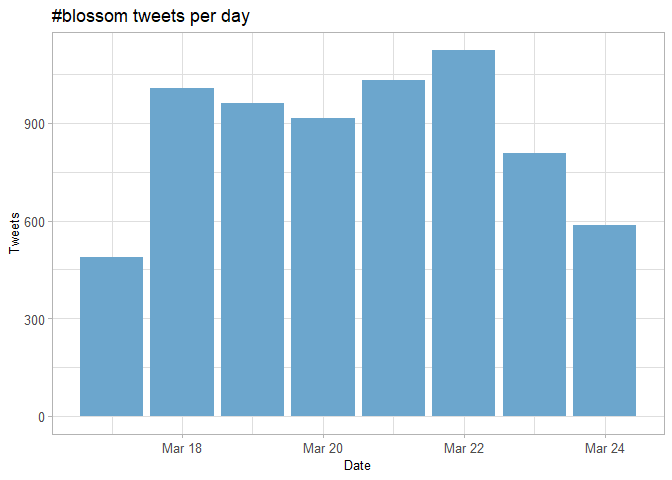
\includegraphics{twitter-blossom-watch-2021_files/figure-latex/tweets-by-day-1.pdf}

\hypertarget{tweets-by-day-and-time}{%
\subsection{Tweets by day and time}\label{tweets-by-day-and-time}}

Filtered for dates March, London time.
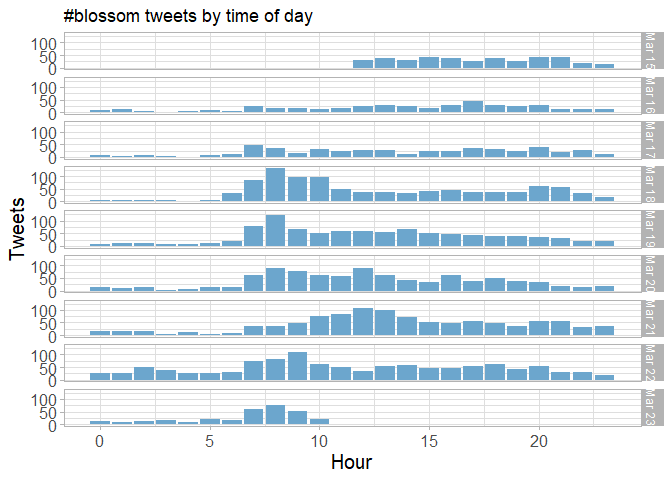
\includegraphics{twitter-blossom-watch-2021_files/figure-latex/tweets-by-day-hour-1.pdf}

\hypertarget{users}{%
\section{Users}\label{users}}

\hypertarget{top-tweeters}{%
\subsection{Top tweeters}\label{top-tweeters}}

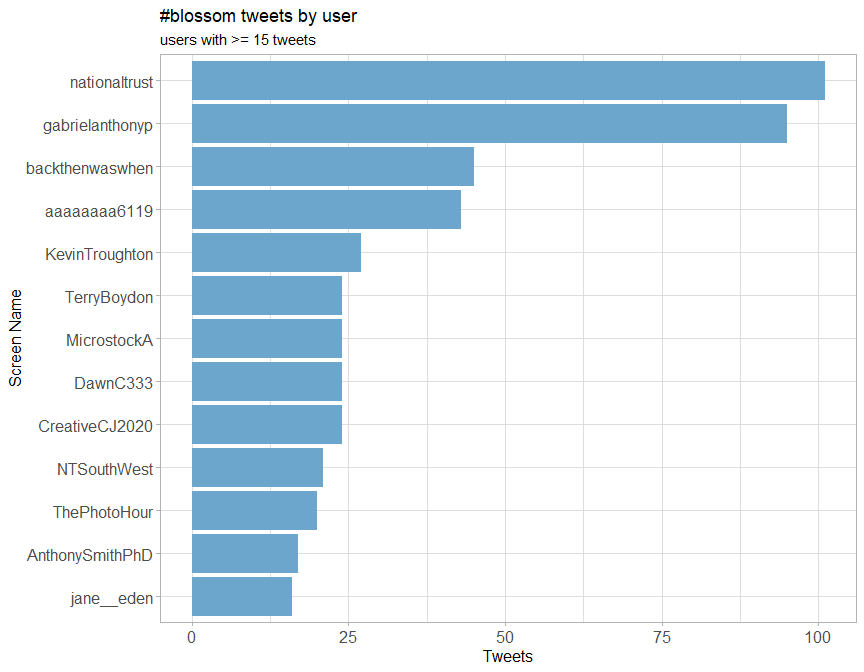
\includegraphics{twitter-blossom-watch-2021_files/figure-latex/tweets-top-users-1.pdf}

\hypertarget{sources}{%
\subsection{Sources}\label{sources}}

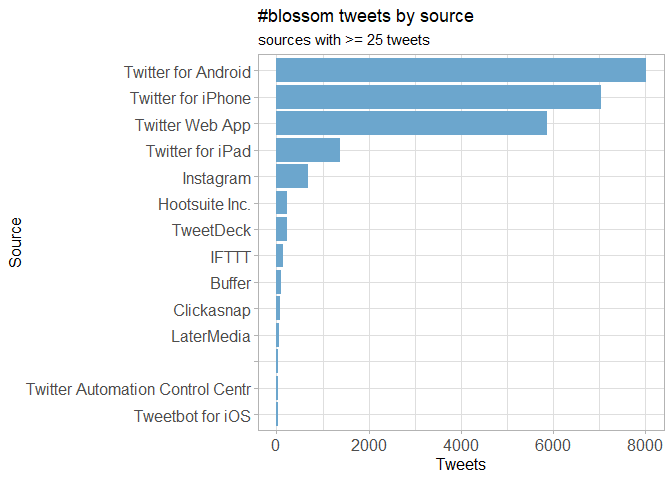
\includegraphics{twitter-blossom-watch-2021_files/figure-latex/tweets-top-sources-1.pdf}

\hypertarget{networks}{%
\section{Networks}\label{networks}}

\hypertarget{replies}{%
\subsection{Replies}\label{replies}}

The ``replies network'', composed from users who reply directly to one
another.

\hypertarget{mentions}{%
\subsection{Mentions}\label{mentions}}

The ``mentions network'', where users mention other users in their
tweets.

\hypertarget{retweets}{%
\section{Retweets}\label{retweets}}

\hypertarget{retweet-proportion}{%
\subsection{Retweet proportion}\label{retweet-proportion}}

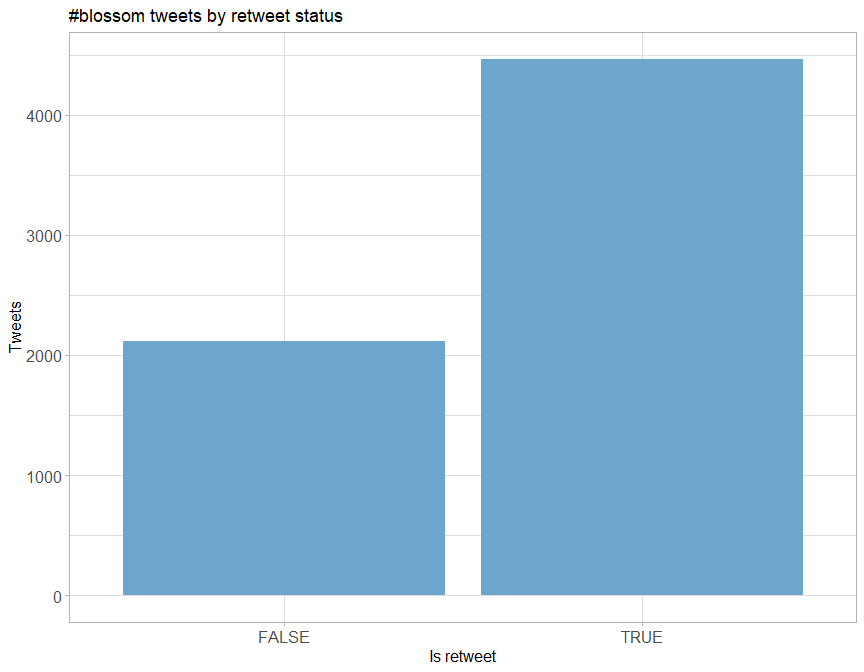
\includegraphics{twitter-blossom-watch-2021_files/figure-latex/is-retweet-1.pdf}

\hypertarget{retweet-count}{%
\subsection{Retweet count}\label{retweet-count}}

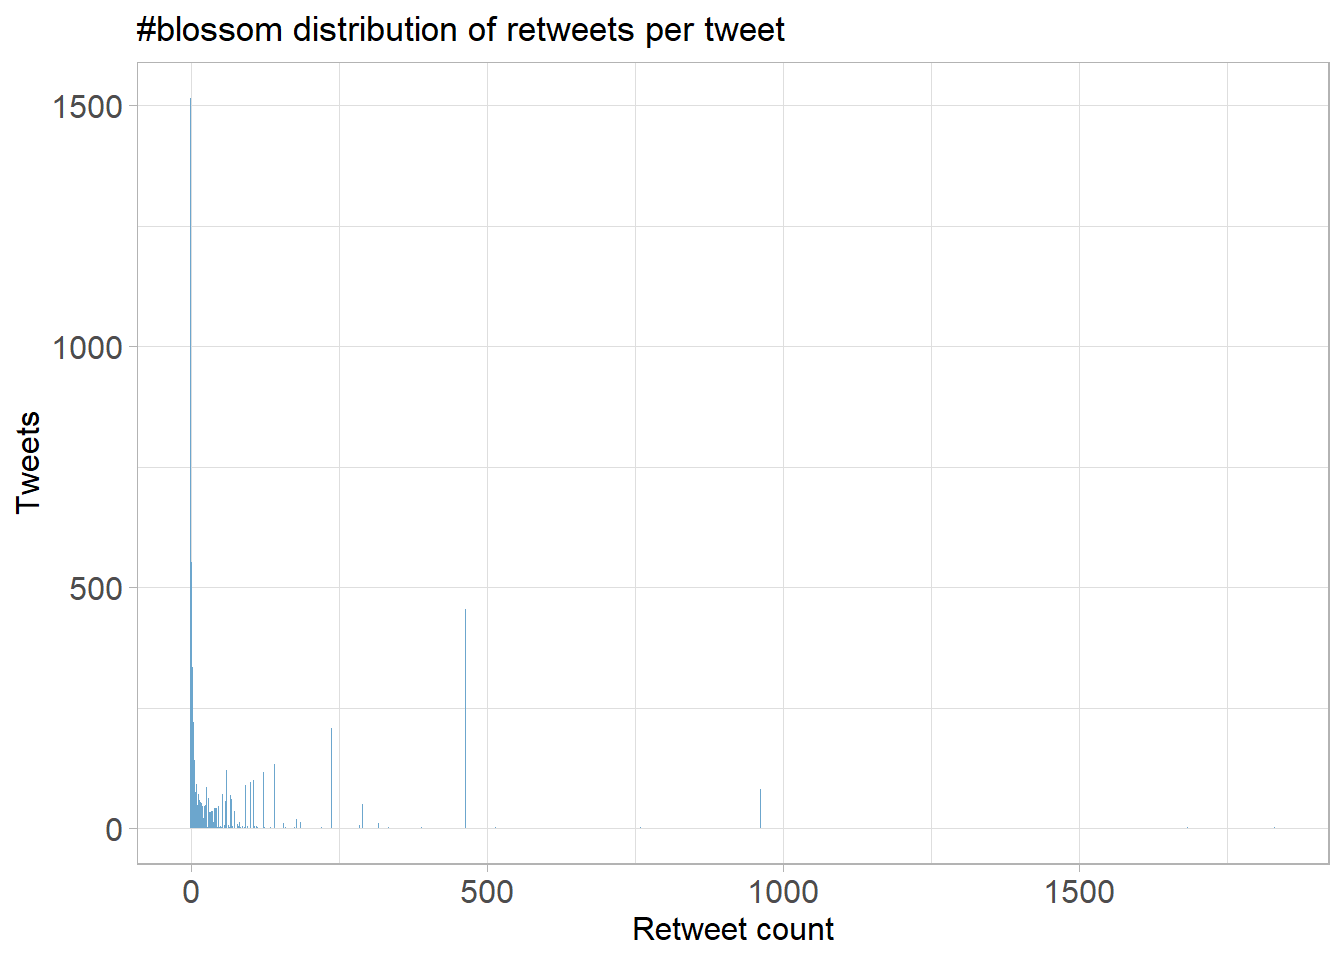
\includegraphics{twitter-blossom-watch-2021_files/figure-latex/retweet-count-1.pdf}

\hypertarget{top-retweets}{%
\subsection{Top retweets}\label{top-retweets}}

\begin{longtable}[]{@{}llr@{}}
\toprule
\begin{minipage}[b]{0.22\columnwidth}\raggedright
screen\_name\strut
\end{minipage} & \begin{minipage}[b]{0.49\columnwidth}\raggedright
text\strut
\end{minipage} & \begin{minipage}[b]{0.20\columnwidth}\raggedleft
retweet\_count\strut
\end{minipage}\tabularnewline
\midrule
\endhead
\begin{minipage}[t]{0.22\columnwidth}\raggedright
nationaltrust\strut
\end{minipage} & \begin{minipage}[t]{0.49\columnwidth}\raggedright
Pause to soak up the sweet scents and soft songs emanating from blossom
branches. These colourful trees are a feast for the senses.
\#BlossomWatch \url{https://t.co/GsXfF5KPAE}\strut
\end{minipage} & \begin{minipage}[t]{0.20\columnwidth}\raggedleft
236\strut
\end{minipage}\tabularnewline
\begin{minipage}[t]{0.22\columnwidth}\raggedright
DrDarrenRFlower\strut
\end{minipage} & \begin{minipage}[t]{0.49\columnwidth}\raggedright
Central Park New York \#spring \#spring2021 \#blossom \#cherry
\url{https://t.co/Oimq2hRU1k}\strut
\end{minipage} & \begin{minipage}[t]{0.20\columnwidth}\raggedleft
139\strut
\end{minipage}\tabularnewline
\begin{minipage}[t]{0.22\columnwidth}\raggedright
nationaltrust\strut
\end{minipage} & \begin{minipage}[t]{0.49\columnwidth}\raggedright
Spring is on the way. Celebrate the arrival of blossom near you with
\#BlossomWatch: \url{https://t.co/TaQxr1YkU8}
\url{https://t.co/kQ93UDZlCP}\strut
\end{minipage} & \begin{minipage}[t]{0.20\columnwidth}\raggedleft
123\strut
\end{minipage}\tabularnewline
\begin{minipage}[t]{0.22\columnwidth}\raggedright
nationaltrust\strut
\end{minipage} & \begin{minipage}[t]{0.49\columnwidth}\raggedright
Everywhere these delicate flowers emerge, they bring delight with them.
Thanks to everyone who's helped spread the joys of blossom so far - keep
the photos coming with \#BlossomWatch. Photos: Joanna A, Catherine A,
Shonali B, Cara W. \url{https://t.co/6znNDEdvKC}\strut
\end{minipage} & \begin{minipage}[t]{0.20\columnwidth}\raggedleft
122\strut
\end{minipage}\tabularnewline
\begin{minipage}[t]{0.22\columnwidth}\raggedright
nationaltrust\strut
\end{minipage} & \begin{minipage}[t]{0.49\columnwidth}\raggedright
If you're lucky enough to spot a hare hopping around, the feeling of
elation will stick with you all day. \#EveryoneNeedsNature
\url{https://t.co/Vpo5aADU9Q}\strut
\end{minipage} & \begin{minipage}[t]{0.20\columnwidth}\raggedleft
100\strut
\end{minipage}\tabularnewline
\begin{minipage}[t]{0.22\columnwidth}\raggedright
nationaltrust\strut
\end{minipage} & \begin{minipage}[t]{0.49\columnwidth}\raggedright
Happily dancing in the breeze, a golden daffodil is full of cheer.
\#EveryoneNeedsNature \url{https://t.co/hSOWdCCnPL}\strut
\end{minipage} & \begin{minipage}[t]{0.20\columnwidth}\raggedleft
96\strut
\end{minipage}\tabularnewline
\begin{minipage}[t]{0.22\columnwidth}\raggedright
nationaltrust\strut
\end{minipage} & \begin{minipage}[t]{0.49\columnwidth}\raggedright
\textless U+0001F338\textgreater\#BlossomWatch\textless U+0001F338\textgreater{}
Lockdowns have changed the nation's relationship with nature for the
better. We are feeling more connected thanks to our daily strolls and
taking more notice of the changing seasons.
\url{https://t.co/JtIkqgUorV}\strut
\end{minipage} & \begin{minipage}[t]{0.20\columnwidth}\raggedleft
93\strut
\end{minipage}\tabularnewline
\begin{minipage}[t]{0.22\columnwidth}\raggedright
nationaltrust\strut
\end{minipage} & \begin{minipage}[t]{0.49\columnwidth}\raggedright
One of life's simple pleasures that can be enjoyed from anywhere.
Engross yourself in the calming colours of a sunrise.
\#EveryoneNeedsNature \url{https://t.co/l5xkDICUPn}\strut
\end{minipage} & \begin{minipage}[t]{0.20\columnwidth}\raggedleft
69\strut
\end{minipage}\tabularnewline
\begin{minipage}[t]{0.22\columnwidth}\raggedright
ampomata\strut
\end{minipage} & \begin{minipage}[t]{0.49\columnwidth}\raggedright
This is my new painting ``Bed Of Roses''. You can check it out here:
\url{https://t.co/GoYnqeM1YY} \#art \#arte \#oleo \#kunst \#oilpainting
\#contemporaryart \#ArtistOnTwitter \#blossom \#flower \#floral \#spring
\#pink \#red \#roses \#field \#artprints \#flowers \#garden
\url{https://t.co/7y9skbUaMs}\strut
\end{minipage} & \begin{minipage}[t]{0.20\columnwidth}\raggedleft
67\strut
\end{minipage}\tabularnewline
\begin{minipage}[t]{0.22\columnwidth}\raggedright
MikeDoylePhotos\strut
\end{minipage} & \begin{minipage}[t]{0.49\columnwidth}\raggedright
Spring colour at Sheffield Park, East Sussex. \#Sussex \#England
\#NationalTrust \#landscape \#landscapephotography \#travel
\#travelphotography \#photo \#photography \#photooftheday
\#NaturePhotography \url{https://t.co/uFdcfnor39}\strut
\end{minipage} & \begin{minipage}[t]{0.20\columnwidth}\raggedleft
60\strut
\end{minipage}\tabularnewline
\bottomrule
\end{longtable}

\hypertarget{favourites}{%
\section{Favourites}\label{favourites}}

\hypertarget{favourite-proportion}{%
\subsection{Favourite proportion}\label{favourite-proportion}}

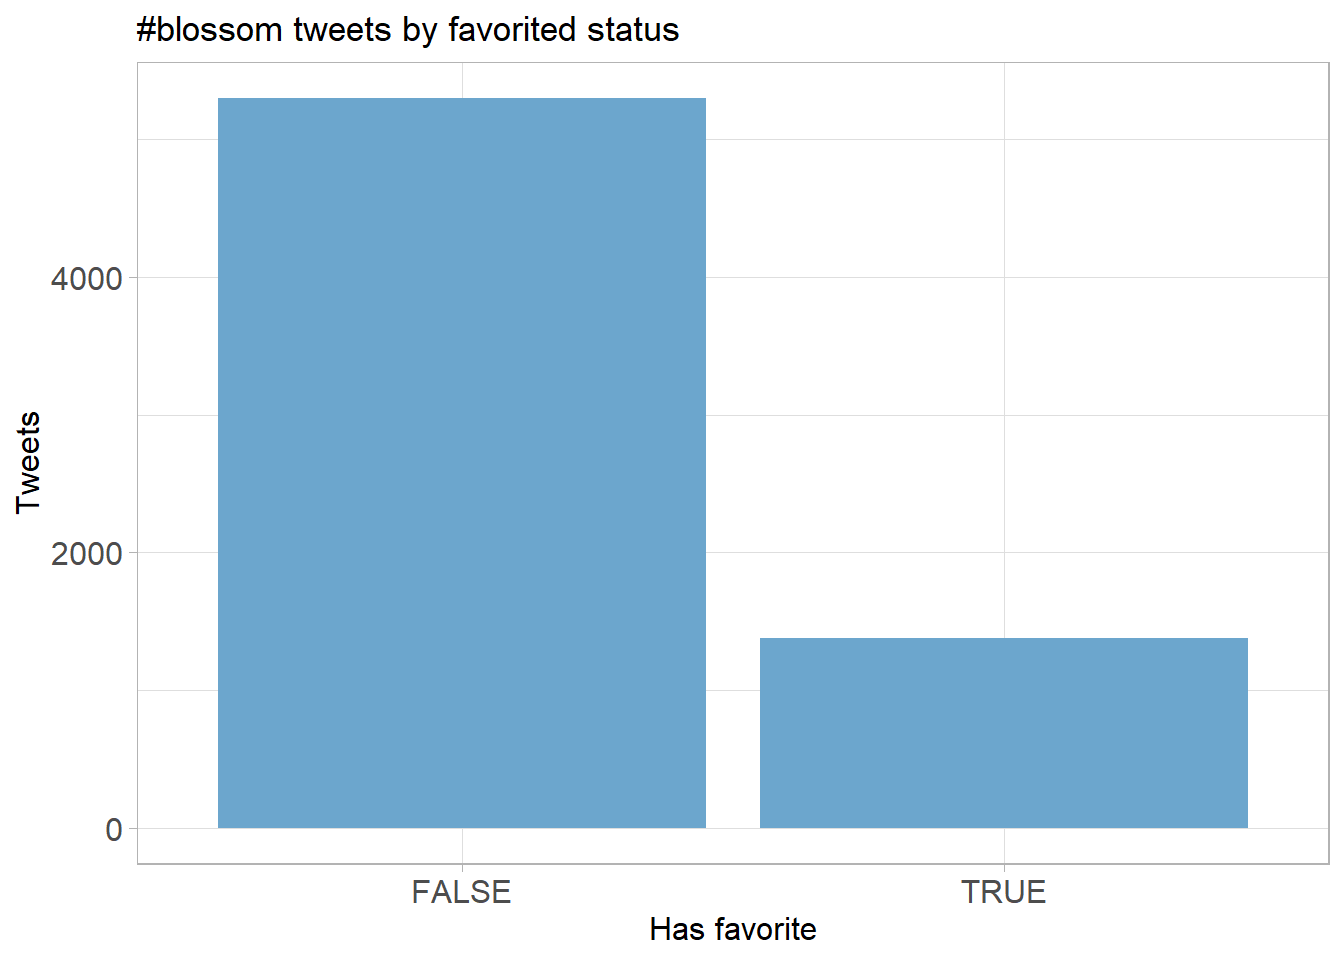
\includegraphics{twitter-blossom-watch-2021_files/figure-latex/has-favorite-1.pdf}

\hypertarget{favourite-count}{%
\subsection{Favourite count}\label{favourite-count}}

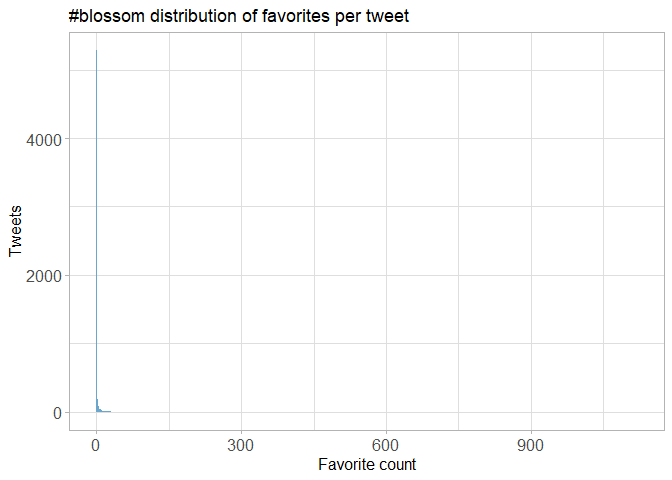
\includegraphics{twitter-blossom-watch-2021_files/figure-latex/favorite-count-1.pdf}

\hypertarget{top-favourites}{%
\subsection{Top favourites}\label{top-favourites}}

\begin{longtable}[]{@{}llr@{}}
\toprule
\begin{minipage}[b]{0.22\columnwidth}\raggedright
screen\_name\strut
\end{minipage} & \begin{minipage}[b]{0.49\columnwidth}\raggedright
text\strut
\end{minipage} & \begin{minipage}[b]{0.21\columnwidth}\raggedleft
favorite\_count\strut
\end{minipage}\tabularnewline
\midrule
\endhead
\begin{minipage}[t]{0.22\columnwidth}\raggedright
nationaltrust\strut
\end{minipage} & \begin{minipage}[t]{0.49\columnwidth}\raggedright
Pause to soak up the sweet scents and soft songs emanating from blossom
branches. These colourful trees are a feast for the senses.
\#BlossomWatch \url{https://t.co/GsXfF5KPAE}\strut
\end{minipage} & \begin{minipage}[t]{0.21\columnwidth}\raggedleft
1107\strut
\end{minipage}\tabularnewline
\begin{minipage}[t]{0.22\columnwidth}\raggedright
DrDarrenRFlower\strut
\end{minipage} & \begin{minipage}[t]{0.49\columnwidth}\raggedright
Central Park New York \#spring \#spring2021 \#blossom \#cherry
\url{https://t.co/Oimq2hRU1k}\strut
\end{minipage} & \begin{minipage}[t]{0.21\columnwidth}\raggedleft
782\strut
\end{minipage}\tabularnewline
\begin{minipage}[t]{0.22\columnwidth}\raggedright
nationaltrust\strut
\end{minipage} & \begin{minipage}[t]{0.49\columnwidth}\raggedright
If you're lucky enough to spot a hare hopping around, the feeling of
elation will stick with you all day. \#EveryoneNeedsNature
\url{https://t.co/Vpo5aADU9Q}\strut
\end{minipage} & \begin{minipage}[t]{0.21\columnwidth}\raggedleft
698\strut
\end{minipage}\tabularnewline
\begin{minipage}[t]{0.22\columnwidth}\raggedright
nationaltrust\strut
\end{minipage} & \begin{minipage}[t]{0.49\columnwidth}\raggedright
Everywhere these delicate flowers emerge, they bring delight with them.
Thanks to everyone who's helped spread the joys of blossom so far - keep
the photos coming with \#BlossomWatch. Photos: Joanna A, Catherine A,
Shonali B, Cara W. \url{https://t.co/6znNDEdvKC}\strut
\end{minipage} & \begin{minipage}[t]{0.21\columnwidth}\raggedleft
692\strut
\end{minipage}\tabularnewline
\begin{minipage}[t]{0.22\columnwidth}\raggedright
nationaltrust\strut
\end{minipage} & \begin{minipage}[t]{0.49\columnwidth}\raggedright
\textless U+0001F338\textgreater\#BlossomWatch\textless U+0001F338\textgreater{}
Lockdowns have changed the nation's relationship with nature for the
better. We are feeling more connected thanks to our daily strolls and
taking more notice of the changing seasons.
\url{https://t.co/JtIkqgUorV}\strut
\end{minipage} & \begin{minipage}[t]{0.21\columnwidth}\raggedleft
565\strut
\end{minipage}\tabularnewline
\begin{minipage}[t]{0.22\columnwidth}\raggedright
nationaltrust\strut
\end{minipage} & \begin{minipage}[t]{0.49\columnwidth}\raggedright
Happily dancing in the breeze, a golden daffodil is full of cheer.
\#EveryoneNeedsNature \url{https://t.co/hSOWdCCnPL}\strut
\end{minipage} & \begin{minipage}[t]{0.21\columnwidth}\raggedleft
531\strut
\end{minipage}\tabularnewline
\begin{minipage}[t]{0.22\columnwidth}\raggedright
nationaltrust\strut
\end{minipage} & \begin{minipage}[t]{0.49\columnwidth}\raggedright
Spring is on the way. Celebrate the arrival of blossom near you with
\#BlossomWatch: \url{https://t.co/TaQxr1YkU8}
\url{https://t.co/kQ93UDZlCP}\strut
\end{minipage} & \begin{minipage}[t]{0.21\columnwidth}\raggedleft
502\strut
\end{minipage}\tabularnewline
\begin{minipage}[t]{0.22\columnwidth}\raggedright
MikeDoylePhotos\strut
\end{minipage} & \begin{minipage}[t]{0.49\columnwidth}\raggedright
Early autumn at Sheffield Park, East Sussex. \#Sussex \#England
\#NationalTrust \#landscape \#landscapephotography \#travel
\#travelphotography \#photo \#photography \#photooftheday
\#NaturePhotography \url{https://t.co/fqSC6f0xMQ}\strut
\end{minipage} & \begin{minipage}[t]{0.21\columnwidth}\raggedleft
470\strut
\end{minipage}\tabularnewline
\begin{minipage}[t]{0.22\columnwidth}\raggedright
MikeDoylePhotos\strut
\end{minipage} & \begin{minipage}[t]{0.49\columnwidth}\raggedright
Spring colour at Sheffield Park, East Sussex. \#Sussex \#England
\#NationalTrust \#landscape \#landscapephotography \#travel
\#travelphotography \#photo \#photography \#photooftheday
\#NaturePhotography \url{https://t.co/uFdcfnor39}\strut
\end{minipage} & \begin{minipage}[t]{0.21\columnwidth}\raggedleft
431\strut
\end{minipage}\tabularnewline
\begin{minipage}[t]{0.22\columnwidth}\raggedright
nationaltrust\strut
\end{minipage} & \begin{minipage}[t]{0.49\columnwidth}\raggedright
Nature's alarm clock is getting louder with each new day as the birds
look to find their spring mates. Which birds are waking you up in the
morning? Photos: Jenni B, @NTCastleWard \#EveryoneNeedsNature
\url{https://t.co/qFLlRf3gL7}\strut
\end{minipage} & \begin{minipage}[t]{0.21\columnwidth}\raggedleft
416\strut
\end{minipage}\tabularnewline
\bottomrule
\end{longtable}

\hypertarget{quotes}{%
\section{Quotes}\label{quotes}}

\hypertarget{quote-proportion}{%
\subsection{Quote proportion}\label{quote-proportion}}

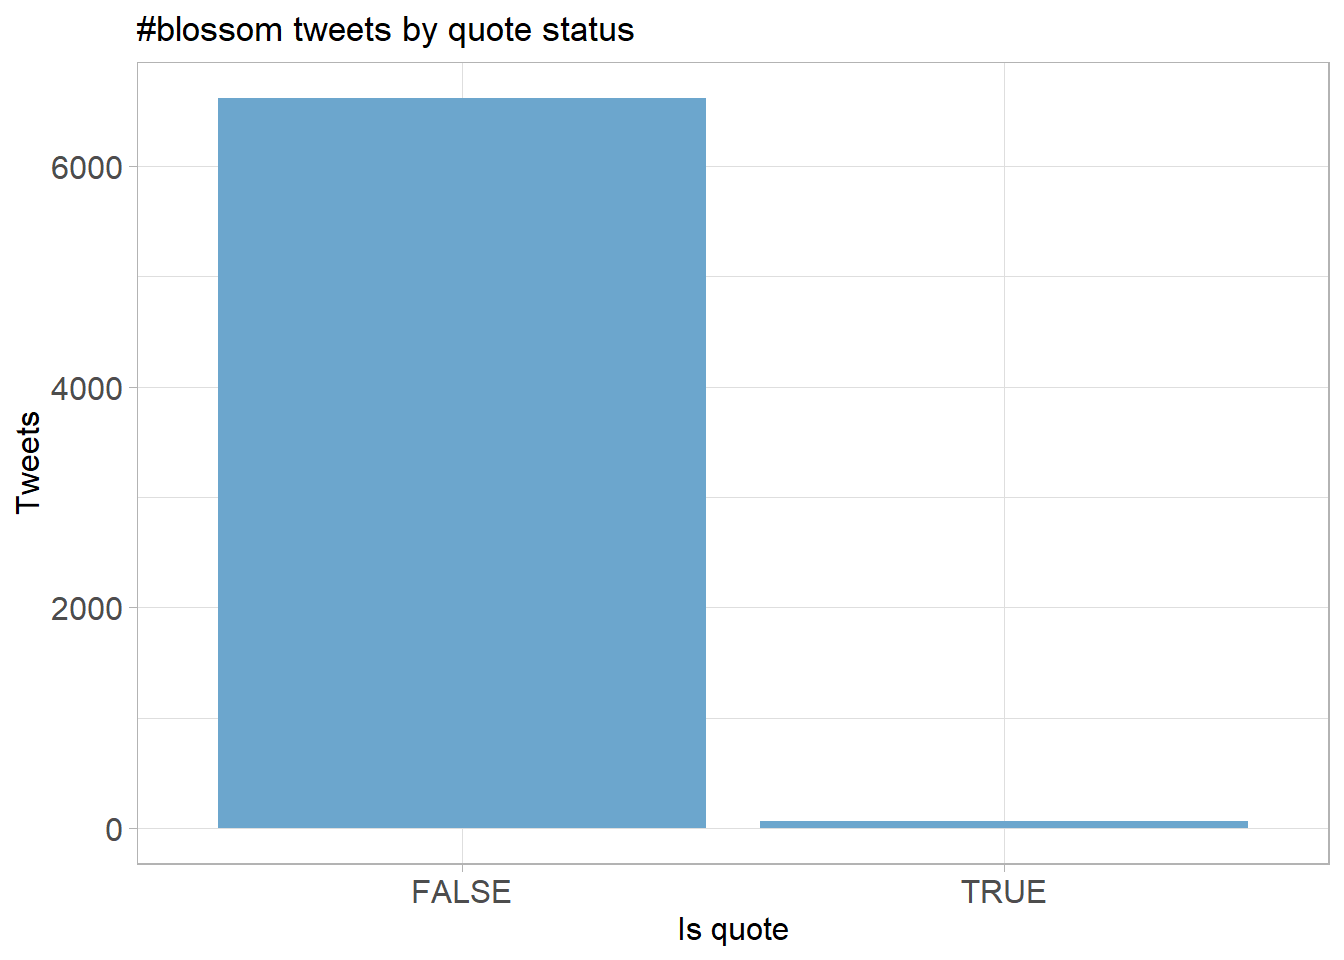
\includegraphics{twitter-blossom-watch-2021_files/figure-latex/is-quote-1.pdf}

\hypertarget{quote-count}{%
\subsection{Quote count}\label{quote-count}}

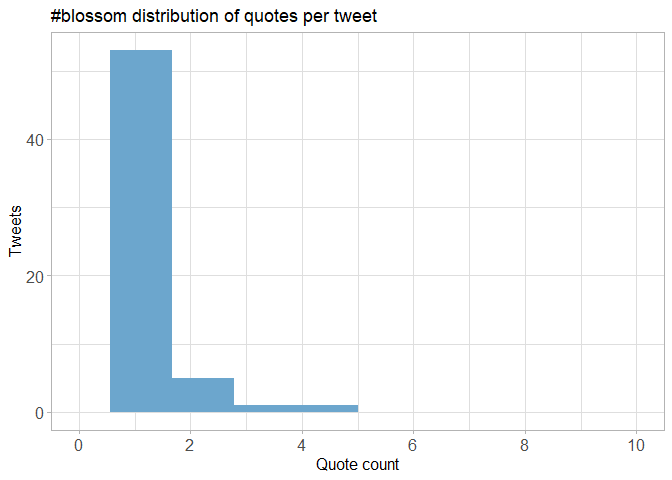
\includegraphics{twitter-blossom-watch-2021_files/figure-latex/quotes-count-1.pdf}

\hypertarget{top-quotes}{%
\subsection{Top quotes}\label{top-quotes}}

Joining, by = ``quoted\_status\_id''

\begin{longtable}[]{@{}llr@{}}
\toprule
\begin{minipage}[b]{0.23\columnwidth}\raggedright
screen\_name\strut
\end{minipage} & \begin{minipage}[b]{0.42\columnwidth}\raggedright
text\strut
\end{minipage} & \begin{minipage}[b]{0.18\columnwidth}\raggedleft
quote\_count\strut
\end{minipage}\tabularnewline
\midrule
\endhead
\begin{minipage}[t]{0.23\columnwidth}\raggedright
wearealtervego\strut
\end{minipage} & \begin{minipage}[t]{0.42\columnwidth}\raggedright
Taking in the \#nature around us\ldots\#andbreathe \#blossomwatch
\#savethebees \#savetheworld \url{https://t.co/9OKBi1ot9E}\strut
\end{minipage} & \begin{minipage}[t]{0.18\columnwidth}\raggedleft
3\strut
\end{minipage}\tabularnewline
\begin{minipage}[t]{0.23\columnwidth}\raggedright
GillianFoxcroft\strut
\end{minipage} & \begin{minipage}[t]{0.42\columnwidth}\raggedright
Wonderful initiative by @nationaltrust Lucky enough to live near
@KedlestonNT where this blackthorn was heralding spring, but blossom is
accessible in our towns and cities too \#BlossomWatch
\url{https://t.co/l3nMn9dvGe} \url{https://t.co/Nri4nxd3vL}\strut
\end{minipage} & \begin{minipage}[t]{0.18\columnwidth}\raggedleft
3\strut
\end{minipage}\tabularnewline
\begin{minipage}[t]{0.23\columnwidth}\raggedright
MedialabGroup\strut
\end{minipage} & \begin{minipage}[t]{0.42\columnwidth}\raggedright
For what is probably the most anticipated spring in decades, we are
incredibly proud to have supported our partner @nationaltrust in
launching their latest Blossom campaign. The National Trust Blossom
campaign runs across TV, national press and digital. \#BlossomWatch
\url{https://t.co/wMan1xCxRM}\strut
\end{minipage} & \begin{minipage}[t]{0.18\columnwidth}\raggedleft
3\strut
\end{minipage}\tabularnewline
\begin{minipage}[t]{0.23\columnwidth}\raggedright
weather2travel\strut
\end{minipage} & \begin{minipage}[t]{0.42\columnwidth}\raggedright
Will you be joining @nationaltrust \#BlossomWatch?
\textless U+0001F338\textgreater\textless U+0001F440\textgreater{}
\#thursdaymorning \#ThoughtForTheDay \#spring \#bliss
\url{https://t.co/aiQYIY1n5N}\strut
\end{minipage} & \begin{minipage}[t]{0.18\columnwidth}\raggedleft
2\strut
\end{minipage}\tabularnewline
\begin{minipage}[t]{0.23\columnwidth}\raggedright
HeiniHeikkil\strut
\end{minipage} & \begin{minipage}[t]{0.42\columnwidth}\raggedright
Mesmerising, refreshing blossom shared by millions in social media
\textless U+0001F338\textgreater\#UKhanami \#BlossomWatch
\url{https://t.co/Ut9p5H0aEL}\strut
\end{minipage} & \begin{minipage}[t]{0.18\columnwidth}\raggedleft
2\strut
\end{minipage}\tabularnewline
\begin{minipage}[t]{0.23\columnwidth}\raggedright
NaturalEngland\strut
\end{minipage} & \begin{minipage}[t]{0.42\columnwidth}\raggedright
Our research shows that nature is more important than ever to us since
the pandemic started. We're taking more notice of small changes in
nature and signs of spring, like beautiful apple blossom. Share your
pictures of blossom with @NationalTrust using
\textless U+0001F338\textgreater\#BlossomWatch
\textless U+0001F338\textgreater{} \url{https://t.co/KlDTIYa46E}\strut
\end{minipage} & \begin{minipage}[t]{0.18\columnwidth}\raggedleft
2\strut
\end{minipage}\tabularnewline
\begin{minipage}[t]{0.23\columnwidth}\raggedright
radiowinch\strut
\end{minipage} & \begin{minipage}[t]{0.42\columnwidth}\raggedright
Spring is on the way. Celebrate the arrival of blossom near you with
\#BlossomWatch share your photos \url{https://t.co/B0TuHmf6Sk}\strut
\end{minipage} & \begin{minipage}[t]{0.18\columnwidth}\raggedleft
2\strut
\end{minipage}\tabularnewline
\begin{minipage}[t]{0.23\columnwidth}\raggedright
LauraSkitt\_\strut
\end{minipage} & \begin{minipage}[t]{0.42\columnwidth}\raggedright
I love blossom trees so much. It reminds me spring is nearly here which
means my birthday is nearly here (end of April, but still!)
\#BlossomWatch \textless U+0001F338\textgreater{}
\url{https://t.co/gB9yiEInEo}\strut
\end{minipage} & \begin{minipage}[t]{0.18\columnwidth}\raggedleft
2\strut
\end{minipage}\tabularnewline
\begin{minipage}[t]{0.23\columnwidth}\raggedright
sheffieldparkNT\strut
\end{minipage} & \begin{minipage}[t]{0.42\columnwidth}\raggedright
Here at @Nationaltrust we are celebrating the delicate clusters of
flowers that are starting to appear on the trees- \#blossomwatch is
here! Have you spotted any blooms festooning the trees? Share your pics
on our blossom map with \#BlossomWatch \url{https://t.co/Uk6EYfJsV4}
\url{https://t.co/T1QMKLUHwo}\strut
\end{minipage} & \begin{minipage}[t]{0.18\columnwidth}\raggedleft
2\strut
\end{minipage}\tabularnewline
\begin{minipage}[t]{0.23\columnwidth}\raggedright
DerbyUniPress\strut
\end{minipage} & \begin{minipage}[t]{0.42\columnwidth}\raggedright
Research @DerbyUni is making important contributions to initiatives
designed to enhance our \#wellbeing and strengthen our relationship with
\#nature, such as @nationaltrust \#BlossomWatch, which has been launched
today. @findingnature \url{https://t.co/c4ZAhGJs1Q}\strut
\end{minipage} & \begin{minipage}[t]{0.18\columnwidth}\raggedleft
2\strut
\end{minipage}\tabularnewline
\bottomrule
\end{longtable}

\hypertarget{media}{%
\section{Media}\label{media}}

\hypertarget{media-count}{%
\subsection{Media count}\label{media-count}}

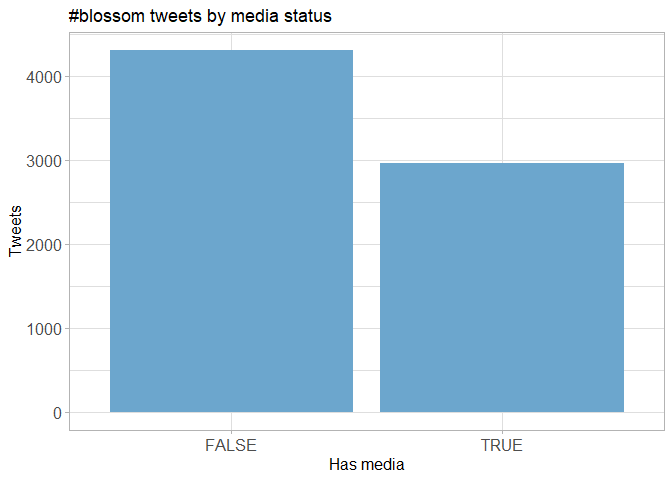
\includegraphics{twitter-blossom-watch-2021_files/figure-latex/has-media-1.pdf}

\hypertarget{top-media}{%
\subsection{Top media}\label{top-media}}

\begin{longtable}[]{@{}llr@{}}
\toprule
\begin{minipage}[b]{0.22\columnwidth}\raggedright
screen\_name\strut
\end{minipage} & \begin{minipage}[b]{0.49\columnwidth}\raggedright
text\strut
\end{minipage} & \begin{minipage}[b]{0.21\columnwidth}\raggedleft
favorite\_count\strut
\end{minipage}\tabularnewline
\midrule
\endhead
\begin{minipage}[t]{0.22\columnwidth}\raggedright
nationaltrust\strut
\end{minipage} & \begin{minipage}[t]{0.49\columnwidth}\raggedright
Pause to soak up the sweet scents and soft songs emanating from blossom
branches. These colourful trees are a feast for the senses.
\#BlossomWatch \url{https://t.co/GsXfF5KPAE}\strut
\end{minipage} & \begin{minipage}[t]{0.21\columnwidth}\raggedleft
1107\strut
\end{minipage}\tabularnewline
\begin{minipage}[t]{0.22\columnwidth}\raggedright
DrDarrenRFlower\strut
\end{minipage} & \begin{minipage}[t]{0.49\columnwidth}\raggedright
Central Park New York \#spring \#spring2021 \#blossom \#cherry
\url{https://t.co/Oimq2hRU1k}\strut
\end{minipage} & \begin{minipage}[t]{0.21\columnwidth}\raggedleft
782\strut
\end{minipage}\tabularnewline
\begin{minipage}[t]{0.22\columnwidth}\raggedright
nationaltrust\strut
\end{minipage} & \begin{minipage}[t]{0.49\columnwidth}\raggedright
If you're lucky enough to spot a hare hopping around, the feeling of
elation will stick with you all day. \#EveryoneNeedsNature
\url{https://t.co/Vpo5aADU9Q}\strut
\end{minipage} & \begin{minipage}[t]{0.21\columnwidth}\raggedleft
698\strut
\end{minipage}\tabularnewline
\begin{minipage}[t]{0.22\columnwidth}\raggedright
nationaltrust\strut
\end{minipage} & \begin{minipage}[t]{0.49\columnwidth}\raggedright
Everywhere these delicate flowers emerge, they bring delight with them.
Thanks to everyone who's helped spread the joys of blossom so far - keep
the photos coming with \#BlossomWatch. Photos: Joanna A, Catherine A,
Shonali B, Cara W. \url{https://t.co/6znNDEdvKC}\strut
\end{minipage} & \begin{minipage}[t]{0.21\columnwidth}\raggedleft
692\strut
\end{minipage}\tabularnewline
\begin{minipage}[t]{0.22\columnwidth}\raggedright
nationaltrust\strut
\end{minipage} & \begin{minipage}[t]{0.49\columnwidth}\raggedright
\textless U+0001F338\textgreater\#BlossomWatch\textless U+0001F338\textgreater{}
Lockdowns have changed the nation's relationship with nature for the
better. We are feeling more connected thanks to our daily strolls and
taking more notice of the changing seasons.
\url{https://t.co/JtIkqgUorV}\strut
\end{minipage} & \begin{minipage}[t]{0.21\columnwidth}\raggedleft
565\strut
\end{minipage}\tabularnewline
\begin{minipage}[t]{0.22\columnwidth}\raggedright
nationaltrust\strut
\end{minipage} & \begin{minipage}[t]{0.49\columnwidth}\raggedright
Happily dancing in the breeze, a golden daffodil is full of cheer.
\#EveryoneNeedsNature \url{https://t.co/hSOWdCCnPL}\strut
\end{minipage} & \begin{minipage}[t]{0.21\columnwidth}\raggedleft
531\strut
\end{minipage}\tabularnewline
\begin{minipage}[t]{0.22\columnwidth}\raggedright
nationaltrust\strut
\end{minipage} & \begin{minipage}[t]{0.49\columnwidth}\raggedright
Spring is on the way. Celebrate the arrival of blossom near you with
\#BlossomWatch: \url{https://t.co/TaQxr1YkU8}
\url{https://t.co/kQ93UDZlCP}\strut
\end{minipage} & \begin{minipage}[t]{0.21\columnwidth}\raggedleft
502\strut
\end{minipage}\tabularnewline
\begin{minipage}[t]{0.22\columnwidth}\raggedright
MikeDoylePhotos\strut
\end{minipage} & \begin{minipage}[t]{0.49\columnwidth}\raggedright
Early autumn at Sheffield Park, East Sussex. \#Sussex \#England
\#NationalTrust \#landscape \#landscapephotography \#travel
\#travelphotography \#photo \#photography \#photooftheday
\#NaturePhotography \url{https://t.co/fqSC6f0xMQ}\strut
\end{minipage} & \begin{minipage}[t]{0.21\columnwidth}\raggedleft
470\strut
\end{minipage}\tabularnewline
\begin{minipage}[t]{0.22\columnwidth}\raggedright
MikeDoylePhotos\strut
\end{minipage} & \begin{minipage}[t]{0.49\columnwidth}\raggedright
Spring colour at Sheffield Park, East Sussex. \#Sussex \#England
\#NationalTrust \#landscape \#landscapephotography \#travel
\#travelphotography \#photo \#photography \#photooftheday
\#NaturePhotography \url{https://t.co/uFdcfnor39}\strut
\end{minipage} & \begin{minipage}[t]{0.21\columnwidth}\raggedleft
431\strut
\end{minipage}\tabularnewline
\begin{minipage}[t]{0.22\columnwidth}\raggedright
nationaltrust\strut
\end{minipage} & \begin{minipage}[t]{0.49\columnwidth}\raggedright
Nature's alarm clock is getting louder with each new day as the birds
look to find their spring mates. Which birds are waking you up in the
morning? Photos: Jenni B, @NTCastleWard \#EveryoneNeedsNature
\url{https://t.co/qFLlRf3gL7}\strut
\end{minipage} & \begin{minipage}[t]{0.21\columnwidth}\raggedleft
416\strut
\end{minipage}\tabularnewline
\bottomrule
\end{longtable}

\hypertarget{most-liked-media-image}{%
\subsubsection{Most liked media image}\label{most-liked-media-image}}

\includegraphics{list("http://pbs.twimg.com/ext_tw_video_thumb/1373173799307345922/pu/img/Qcm5UVfXdZyyCNjR.jpg")}

\hypertarget{tweet-text}{%
\section{Tweet text}\label{tweet-text}}

The 250 words used 3 or more times. Words removed: blossom,
blossomwatch, nationaltrust, everyoneneedsnature.

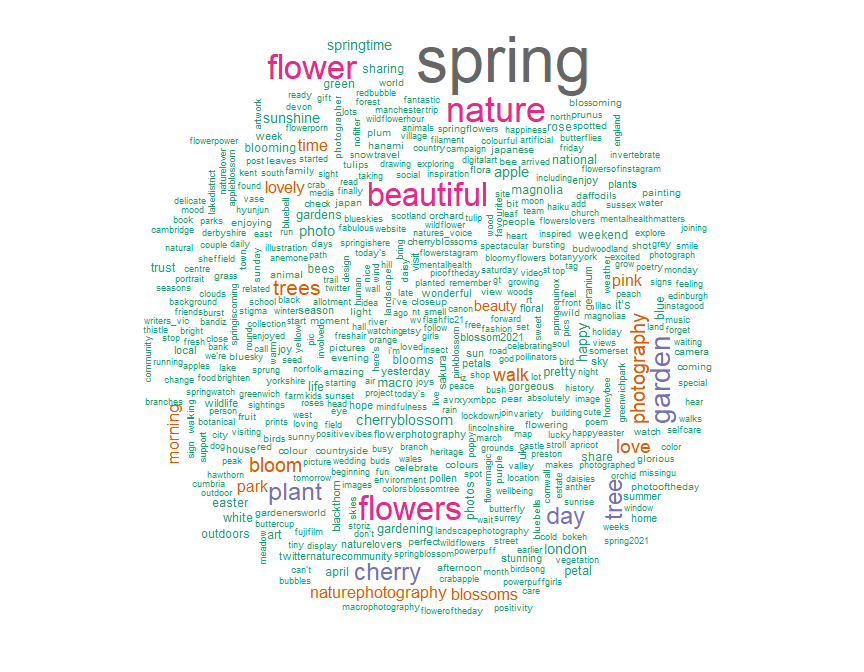
\includegraphics{twitter-blossom-watch-2021_files/figure-latex/count-words-1.pdf}

\hypertarget{tweets-by-tweet-length}{%
\subsection{Tweets by Tweet Length}\label{tweets-by-tweet-length}}

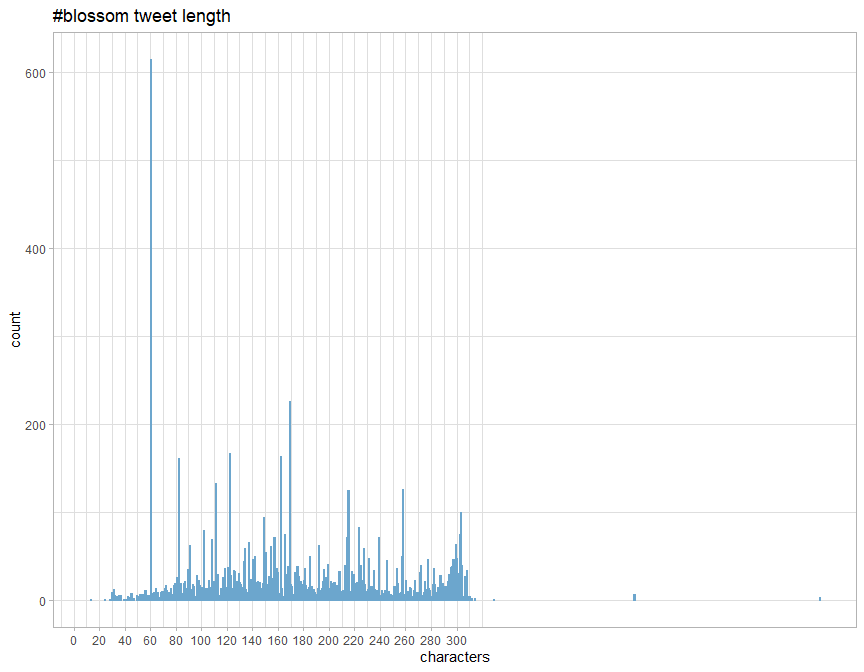
\includegraphics{twitter-blossom-watch-2021_files/figure-latex/count-tweet-length-1.pdf}

\hypertarget{blossom-sentiment-analysis---visualisation}{%
\subsection{Blossom Sentiment Analysis -
Visualisation}\label{blossom-sentiment-analysis---visualisation}}

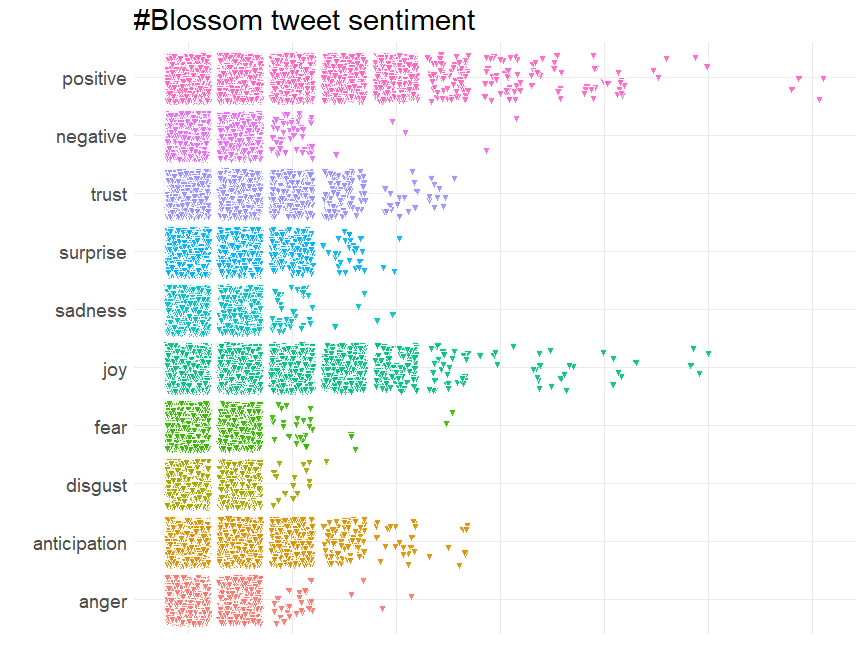
\includegraphics{twitter-blossom-watch-2021_files/figure-latex/unnamed-chunk-2-1.pdf}

\end{document}
